\documentclass[conference]{IEEEtran}
\IEEEoverridecommandlockouts
% The preceding line is only needed to identify funding in the first footnote. If that is unneeded, please comment it out.
\usepackage{cite}
\usepackage[utf8]{inputenc}
\usepackage[dvipsnames]{xcolor}
\usepackage{varwidth}
\usepackage{amsmath,amssymb,amsfonts}
\usepackage{algorithmic}
\usepackage{graphicx}
\usepackage{textcomp}
\usepackage{bm}
\usepackage{bbm}
\usepackage{empheq}
\usepackage{etoolbox}
\usepackage{hyperref}
\usepackage{attachfile}



\def\BibTeX{{\rm B\kern-.05em{\sc i\kern-.025em b}\kern-.08em
    T\kern-.1667em\lower.7ex\hbox{E}\kern-.125emX}}
    
    
\DeclareMathOperator*{\argmin}{arg\,min}
\DeclareMathOperator*{\grad}{grad}
\let\div\undefined
\DeclareMathOperator*{\div}{div}

\newcommand*{\E}[1]{\ensuremath{\mathbb{E}\left[#1\right]}}
\renewcommand*{\P}[2][]{\ensuremath{\mathbb{P}#1\left(#2\right)}}
\newcommand*{\Var}[1]{\ensuremath{\text{Var}\left(#1\right)}}
\newcommand*{\Cov}[2]{\ensuremath{\text{Cov}\left({#1}, {#2}\right)}}
\newcommand*{\Corr}[1]{\ensuremath{\text{Corr}\left(#1\right)}}
\newcommand*{\sd}[1]{\ensuremath{\sigma_{#1}}}
\newcommand*{\card}[1]{\ensuremath{\lvert#1\rvert}}
\newcommand*{\warn}[1]{\textcolor{OrangeRed}{#1}}
\newcommand*{\important}[1]{\fcolorbox{BurntOrange}{BurntOrange!10!White}{\begin{varwidth}{\textwidth}
#1
\end{varwidth}}}
\renewcommand*{\d}[1]{\ensuremath{\mathrm{d}#1}}
\newcommand*{\dist}{\sim}
\newcommand*{\indicator}{\ensuremath{\mathbb{1}}}
\newcommand*{\reals}{\ensuremath{\mathbb{R}}}
\newcommand*{\integers}{\ensuremath{\mathbb{Z}}}
\newcommand*{\naturals}{\ensuremath{\mathbb{N}}}
\newcommand*{\abs}[1]{\ensuremath{\left\lvert#1\right\rvert}}
\newcommand*{\floor}[1]{\ensuremath{\lfloor#1\rfloor}}
\newcommand*{\inclimg}[2][]{\begin{figure}[H]\centering\includegraphics[max width=0.9\textwidth,keepaspectratio]{#2}#1\end{figure}}
\newcommand*{\diff}[2]{\ensuremath{\frac{\d}{\d{#2}}{#1}}}
\newcommand*{\pdiff}[2]{\ensuremath{\frac{\partial}{\partial{#2}}{#1}}}
\newcommand*{\ddiff}[2]{\ensuremath{\frac{\delta}{\delta{#2}}{#1}}}
\newcommand*{\mdiff}[3]{\ensuremath{\frac{\d{^{#3}}}{\d{#2}^{#3}}{#1}}}
\newcommand*{\pmdiff}[3]{\ensuremath{\frac{\partial{^{#3}}}{\partial{#2}^{#3}}{#1}}}

\newcommand*{\at}[1]{\ensuremath{\biggr\rvert_{#1}}}
\renewcommand*{\i}{\ensuremath{\text{i}}}
\newcommand{\distlike}{\ensuremath{\sim}}
\newcommand{\normaldist}[2]{\ensuremath{\mathcal{N}\left(#1, #2\right)}}
\newcommand{\asnormaldist}[2]{\distlike\normaldist{#1}{#2}}
\renewcommand*{\vec}[1]{\ensuremath{{\bm{#1}}}}
\newcommand*{\mat}[1]{\vec{#1}}
\newcommand*{\transpose}[1]{{#1}^{\mkern-1.5mu\mathsf{T}}}
\newcommand*{\transposeinvert}[1]{{#1}^{\mkern-1.5mu\mathsf{-T}}}
\newcommand*{\invert}[1]{{#1}^{-1}}
\newcommand*{\tvec}[1]{\transpose{\vec{#1}}}
\newcommand*{\tmat}[1]{\tvec{#1}}
\newcommand*{\rgramian}[1]{{#1}\transpose{#1}}
\newcommand*{\lgramian}[1]{\transpose{#1}{#1}}
\renewcommand*{\indicator}{\ensuremath{\mathbbm{1}}}
\newcommand*{\invmat}[1]{\ensuremath{\invert{\mat{#1}}}}
\newcommand*{\iprod}[3]{\ensuremath{\ifstrempty{#1}{\transpose{#2} {#3}}{\transpose{#1} {#2} {#3}}}}
\newcommand*{\ciprod}[2]{\ensuremath{\left\langle{#1},{#2}\right\rangle}}
\newcommand*{\miprod}[2]{\iprod{#1}{#2}{#1}}
\newcommand*{\enm}[1]{\left\langle{#1}\right\rangle}
\DeclareMathOperator*{\hmean}{hm}
%\newcommand*{\grad}{\mathrm{grad}}
%\renewcommand*{\div}{\mathrm{div}}
\newcommand*{\bigO}[1]{\ensuremath{\mathcal{O}\left({#1}\right)}}
\begin{document}

\title{Report for the semester thesis ``Development of a Monte Carlo algorithm for optimal control problems''}

\author{\IEEEauthorblockN{Stefano Weidmann}
\IEEEauthorblockA{\textit{Institute of Fluid Dynamics} \\
\textit{ETH Zurich}\\
Zurich, Switzerland \\
\href{mailto:stefanow@student.ethz.ch}{stefanow@student.ethz.ch}}}
%\and
%\IEEEauthorblockN{2\textsuperscript{nd} Given Name Surname}
%\IEEEauthorblockA{\textit{dept. name of organization (of Aff.)} \\
%\textit{name of organization (of Aff.)}\\
%City, Country \\
%email address}
%\and
%\IEEEauthorblockN{3\textsuperscript{rd} Given Name Surname}
%\IEEEauthorblockA{\textit{dept. name of organization (of Aff.)} \\
%\textit{name of organization (of Aff.)}\\
%City, Country \\
%email address}
%\and
%\IEEEauthorblockN{4\textsuperscript{th} Given Name Surname}
%\IEEEauthorblockA{\textit{dept. name of organization (of Aff.)} \\
%\textit{name of organization (of Aff.)}\\
%City, Country \\
%email address}
%\and
%\IEEEauthorblockN{5\textsuperscript{th} Given Name Surname}
%\IEEEauthorblockA{\textit{dept. name of organization (of Aff.)} \\
%\textit{name of organization (of Aff.)}\\
%City, Country \\
%email address}
%\and
%\IEEEauthorblockN{6\textsuperscript{th} Given Name Surname}
%\IEEEauthorblockA{\textit{dept. name of organization (of Aff.)} \\
%\textit{name of organization (of Aff.)}\\
%City, Country \\
%email address}
%}

\maketitle

\begin{abstract}
The Monte-Carlo adjoint algorithm described in \cite{unsteady} has been applied to a variant of the \emph{quarter five spot configuration} found in petroleum engineering literature \cite{quarterFiveSpot}.
Results have been unsatisfactory due to lack of an appropriate preconditioner.
\end{abstract}


\section{Introduction}
This report aims to apply the Monte-Carlo adjoint algorithm described in \cite{unsteady} to a variant of problem known as \emph{quarter five spot configuration} in petroleum engineering literature \cite{quarterFiveSpot}. The set up is described in section \ref{problemDescription}.
Numerical experiments and a discussion follow in section \ref{experiments}. Possible ways how to proceed are given in section \ref{possibleSolutions}. Derivatives needed for the implementation of the Monte-Carlo adjoint algorithm are given in the appendix in subsection \ref{quantitiesNeeded}. The source code can be obtained by visiting the repository at
\href{https://gitlab.ethz.ch/stefanow/mcadjoint}{https://gitlab.ethz.ch/stefanow/mcadjoint}.

The main advantage of the Monte-Carlo adjoint algorithm in comparison to the better known \emph{checkpointing} scheme proposed by Griewank and Walter \cite{checkpointing} lies in its forward-in-time nature. Instead of having to store or recompute solutions, the adjoint equation can be solved in lockstep with the forward one.
In principle, it is an application of the classic Monte-Carlo linear solver developed in \cite{forsythe} applied to the adjoint linear system of equations.

\section{Problem description}
\label{problemDescription}
We model a cross section of an oil field as a two dimensional square $\Omega := [0, 1]^2.$ In the field, there are two phases: water and oil. 
At the lower left corner $\vec{x}_\text{drill} := (0, 0)$, we know the pressure $p_\text{drill}(t)$ and the water inflow $Q_\text{w, drill}(t).$ Opposite of that, at $\vec{x}_\text{well} := (1, 1)$ a well is located.
There we can measure the pressure $p_\text{well}(t)$ as well as the total volumetric outflow \begin{equation}
{Q}_\text{tot}(t) := {Q}_\text{o}(t) + {Q}_\text{w}(t) = Q_\text{w, drill}(t)
\end{equation} per unit depth.
There is no flow through the boundary of the domain except at the drill location $\vec{x}_\text{drill}$ and the well location $\vec{x}_\text{well}.$

The flow rates for both phases are described by Darcy's law
\begin{equation}
\label{flowrateWater}
\vec{v}_\text{w} = -\frac{k k_\text{rel, w}}{\mu_\text{w}} \grad(p),
\end{equation}
for water and
\begin{equation}
\label{flowrateOil}
\vec{v}_\text{o} = -\frac{k k_\text{rel, o}}{\mu_\text{o}} \grad(p)
\end{equation}
for oil.
Here, $p(\vec{x}, t)$ is the pressure, $\mu_\text{o}$, $\mu_\text{w}$ are dynamic viscosities for oil and water, $k(\vec{x}, t)$ is the permeability.
$k_\text{rel, o}(S)$, $k_\text{rel, w}(S)$ are relative permeabilities and are assumed to depend quadratically on the saturation of water $S_\text{w} \in [0, 1]$ and the saturation of oil $S_\text{o} \in [0, 1]$:
\begin{align}
\label{relativePermeabilityModel}
k_\text{rel, o} &= S_\text{o}^2\\
k_\text{rel, w} &= S_\text{w}^2.
\end{align}
The saturations are linked by the constitutive relation
\begin{equation}
S_\text{o} + S_\text{w} = 1.
\end{equation}

$\vec{v}_\text{o}(\vec{x}, t)$, $\vec{v}_\text{w}(\vec{x}, t)$ finally are the volumetric flow rates per unit area (Darcy velocities).

The saturation $S$ is not assumed constant but instead is transported according to the equation
\begin{equation}
\label{stransp}
\phi\pdiff{S_\text{w}}{t} + \div(\vec{v}_\text{w}) = q_\text{w}.
\end{equation}
The term
\begin{equation}
q_\text{w} := Q_\text{w}\delta(\vec{x} - \vec{x}_\text{well})
\end{equation}
describes a line sink of water located at the well.
Similarly, we use
\begin{align}
q_\text{o} &:= Q_\text{o}\delta(\vec{x} - \vec{x}_\text{well}) \\
q_\text{tot} &:= q_\text{o} + q_\text{w}.
\end{align}
$\phi$ is the porosity of the rock which is assumed to be constant over the domain.

Conservation of the total mass then reads
\begin{equation}
\label{conservationOfMass}
\div(\vec{v}_\text{tot}) = q_\text{tot},
\end{equation}
where
\begin{equation}
\vec{v}_\text{tot} := \vec{v}_\text{o} + \vec{v}_\text{w}
\end{equation}
is the total Darcy velocity.

We then introduce the mobilities
\begin{align}
\label{lambdas}
\lambda_\text{o} &:= \frac{k k_\text{rel, o}}{\mu_\text{o}} \\
\lambda_\text{w} &:= \frac{k k_\text{rel, w}}{\mu_\text{w}} \\
\lambda_\text{tot} &:= \lambda_\text{o} + \lambda_\text{w}.
\end{align}

Substituting in the $\lambda$ from \eqref{lambdas} into Darcy's law \eqref{flowrateOil}, \eqref{flowrateWater} and adding both sides of the results we get the total Darcy's law

\begin{equation}
\label{flowrateTotal}
\vec{v}_\text{tot} = - \lambda_\text{tot} \grad(p).
\end{equation}

Plugging this \eqref{flowrateTotal} into the conservation of mass \eqref{conservationOfMass} leads to the pressure equation
\begin{empheq}[box=\fbox]{equation}
\label{pressurePoisson}
\div(\lambda_\text{tot}\grad(p)) = -q_\text{tot}.
\end{empheq}

Comparing the total Darcy's law \eqref{flowrateTotal} and the Darcy's law for water \eqref{flowrateWater}, we see that
\begin{equation}
\vec{v}_\text{w} = \frac{\lambda_\text{w}}{\lambda_\text{tot}} \vec{v}_\text{tot}.
\end{equation}

We then plug in the model for the relative permeabilities in terms of the saturations \eqref{relativePermeabilityModel}, to get the final for of saturation transport equation

\begin{empheq}[box=\fbox]{equation}
\label{saturationEquation}
\pdiff{S_\text{w}}{t} + \div\left(f(S_\text{w}) \vec{v}_\text{tot})\right) = \frac{q_\text{w}}{\phi},
\end{empheq}
where $f$ is the flux function
\begin{empheq}[box=\fbox]{equation}
f(S_\text{w}) := \frac{S_\text{w}^2 / \phi}{S_\text{w}^2 + (1-S_\text{w})^2 \mu_\text{w} / \mu_\text{o}}.
\end{empheq}

\subsection{Boundary and initial conditions}
We assume the initial saturation of water to be given,
which is $S_\text{w}(\vec{x}, 0).$
For the pressure equation we use homogeneous Neumann boundary conditions (no flow), i.e.
\begin{equation}
\grad(p) = p_0 \begin{pmatrix} \delta(x - x_w) \\ \delta(y - y_w), \end{pmatrix},
\end{equation}
where we choose $p_0$ such that the compatibility condition
\begin{equation}
\int_\Omega q_\text{tot} \d{A} \overset{!}{=} \int_{\partial\Omega} \lambda_\text{tot} \iprod{}{\grad(p)}{\vec{n}} \d{l}
\end{equation}
is satisfied.

\subsection{What to optimize?}
To test the Monte-Carlo adjoint method, we want to match the pressure at the drill, i.e.
\begin{equation}
\label{costFunction}
c(T) := \int_0^T \biggr(p_\text{drill}(t) - \tilde{p}_\text{drill}(t)\biggr)^2 \d{t},
\end{equation}
where the variables with a tilde denote computed quantities and $T$ is a final time.

\subsection{What do we control?}
We control the log-permeabilities $\ln(k)$, as these are hard to measure.
Controlling the logarithms $\ln(k)$ instead of just the permeabilities $k$ has the added advantage of being able to cover a wider range of permeabilities and implicitly making sure that the permeabilities are always positive regardless of the choice of optimizer.

\section{Discretization}
We discretize the square domain $\Omega$ with $N \times N$ square finite volumes, thus getting a mesh width of $h := 1/N$.

An overview of the discretization technique is given in the following procedure:
\begin{enumerate}
	\item Solve the pressure equation \eqref{pressurePoisson} as detailed in subsection \ref{discPressurePoisson}
	\item Compute the total Darcy velocity as in \eqref{flowrateTotal}, using the same approximation of the gradient as in the first step
	\item Solve the saturation equation \eqref{saturationEquation} as in subsection \ref{discSaturationEquation}
	\item Update the relative permeabilities according to \eqref{relativePermeabilityModel} and repeat
\end{enumerate}

\subsection{Discretizing the pressure Poisson equation}
\label{discPressurePoisson}
Averaging the pressure Poisson equation \eqref{pressurePoisson} over such a finite volume $K$, and using the divergence theorem leads to
\begin{equation}
\label{finiteVolumes}
\frac{1}{h^2} \int_{\partial K} \lambda_\text{tot} \iprod{}{\grad(p)}{\vec{n}} \d{l} = -\frac{1}{h^2} \int_K q_\text{tot} \d{A}.
\end{equation}
Using the four boundaries $N$orth, $E$ast, $S$outh and $W$est of the finite volume $K$, we approximate \eqref{finiteVolumes} as
\begin{multline}
\frac{1}{h}\biggr( (\lambda_\text{tot} \ddiff{p}{x})\lvert_\text{E} - (\lambda_\text{tot} \ddiff{p}{x})\lvert_\text{W} \\+ (\lambda_\text{tot}\ddiff{p}{y})\lvert_\text{N}
- \ddiff{p}{y})\lvert_\text{S} \biggr) \\= - \frac{Q_\text{tot}}{h^2} \cdot \begin{cases} 1, &\text{if } K \text{ is the finite volume nearest to the well} \\
0, & \text{otherwise} \end{cases}
\end{multline}

$\ddiff{\cdot}{\cdot}$ denote the standard finite difference quotients, i.e.
\begin{align}
\label{differenceQuotients}
\ddiff{p}{x}\lvert_\text{E} &= \frac{1}{h}(p_R - p_K) \\
\ddiff{p}{x}\lvert_\text{W} &= \frac{1}{h}(p_K - p_D) \\
\ddiff{p}{y}\lvert_\text{N} &= \frac{1}{h}(p_U - p_K) \\
\ddiff{p}{y}\lvert_\text{S} &= \frac{1}{h}(p_K - p_D).
\end{align}
Here, $U$ stands for the upper neighbor of $K$, $D$ for the lower (down), $R$ for the right and $L$ for the left.
$p_K$ is the pressure at the center of the volume, which is taken to be the same as the volume averaged $\bar{p}$, as our scheme is just first order.

The total mobilities $\lambda_\text{tot}$ at the boundaries are approximated by the harmonic mean of the total mobilities inside the adjacent finite volumes as
\begin{align}
\label{harmonicMeans}
\lambda_\text{tot}\lvert_\text{E} &\approx \hmean(\lambda_\text{tot}\lvert_K, \lambda_\text{tot}\lvert_R) \\
\lambda_\text{tot}\lvert_\text{W} &\approx \hmean(\lambda_\text{tot}\lvert_K, \lambda_\text{tot}\lvert_L) \\
\lambda_\text{tot}\lvert_\text{N} &\approx \hmean(\lambda_\text{tot}\lvert_K, \lambda_\text{tot}\lvert_U) \\
\lambda_\text{tot}\lvert_\text{S} &\approx \hmean(\lambda_\text{tot}\lvert_K, \lambda_\text{tot}\lvert_D),
\end{align}
where \begin{equation}
\hmean(a, b) = 2ab/(a+b).
\end{equation}
We take the harmonic average instead of the arithmetic average for the following reasons as is detailed also in \cite{perminc}.
The total pressure drop over two adjacent cells is given as
\begin{equation}
\Delta p_\text{tot} = \Delta p_1 + \Delta p_2,
\end{equation}
plugging in a simplified version of Darcy's law which reads
\begin{equation}
\Delta p  = \frac{-v\mu h}{k},
\end{equation}
and canceling terms we have that
\begin{equation}
\frac{1}{k_\text{avg}} = \frac{1}{2}\left(\frac{1}{k_1} + \frac{1}{k_2}\right),
\end{equation}
which is a harmonic average for $k$ and so also for $\lambda.$

The discretized pressure Poisson equation reads
\begin{multline}
T_E (p_K - p_R) + T_W (p_K - p_L) \\+ T_N ( p_K - p_U) + T_S (p_K - p_D) \\= {Q_\text{tot}} \cdot \begin{cases} 1, &\text{if } K \text{ is the finite volume nearest to the well} \\
0, & \text{otherwise} \end{cases},
\end{multline}

where \begin{equation}
T_N = \hmean(\lambda_\text{tot}\lvert_K, \lambda_\text{tot}\lvert_U),
\end{equation}
and so on.

\subsection{Discretizing the saturation equation}
\label{discSaturationEquation}
The finite volume reformulation of the saturation equation \eqref{saturationEquation} leads to the following:
\begin{multline}
\label{saturationEquationFV}
\pdiff{\frac{1}{h^2} \int_K S_\text{w} \d{A}}{t} \\+ \frac{1}{h}\biggr((f(S_\text{w})v_{\text{tot }, x})\lvert_E - (f(S_\text{w})v_{\text{tot }, x})\lvert_W \\+ (f(S_\text{w})v_{\text{tot }, y})\lvert_N - (f(S_\text{w})v_{\text{tot }, y})\lvert_S\biggr) \\=
\frac{Q_\text{w}}{h^2 \phi} \cdot \begin{cases} 1, &\text{if } K \text{ is the finite volume nearest to the well} \\0, &\text{otherwise}\end{cases}
\end{multline}

We identify the volume average
\begin{equation}
\frac{1}{h^2} \int_K S_\text{w} \d{A} =: S_K,
\end{equation}
with the saturation at the center of the volume $S_K$. This is legit, as our scheme is just first order.

For the total Darcy velocity $\vec{v}_\text{tot}$ we use the same discretization of the pressure gradients as in the pressure equation, \eqref{differenceQuotients}.
This makes it available at the boundaries ($N$, $S$, $E$, $W$), as required by \eqref{saturationEquationFV}.

For the flux function $f$ at the boundaries, we use an upwind discretization. The standard formulation can be simplified by noting that \begin{equation}
\diff{f}{S_\text{w}} > 0
\end{equation}
and so instead of the advection velocity
\begin{equation}
\pdiff{(f \cdot \vec{v}_\text{tot})}{S_\text{w}}
\end{equation}
we can use the Darcy velocity $\vec{v}_\text{tot}.$
We remember that this requires fixing the total Darcy velocity $\vec{v}_\text{tot}$ to be independent of the saturation $S_\text{w}$

For timestepping of the saturation equation \eqref{saturationEquationFV} , we use explicit Euler, as this simplifies the Jacobian used in the Monte-Carlo adjoint.

\subsection{Discretizing the cost function}
The cost function \eqref{costFunction} is discretized as a sum of squares over the timesteps, i.e.

\begin{equation}
F := \sum_{i=1}^{n} (p_\text{drill}(i\Delta t) - p_\text{drill cell}^{(i)})^2,
\end{equation}
where $p_\text{drill cell}$ is the computed pressure at the drill cell, $p_\text{drill}$ is the provided pressure at the drill in the $i$-th timelevel, and $\Delta t$ is the timestep.

\subsection{Formal definition of the residuals for the Monte-Carlo adjoint solver}
First, we define the pressure residuals
\begin{multline}
\Pi_K^{(i)} := \begin{cases} p_K^{(i)} - p_\text{well}(i\Delta t), & \text{if } K \text{ is the cell}\\&\text{nearest to the well}\\T_E^{(i-1)} (p_K^{(i)} - p_R^{(i)}) \\+ T_W^{(i-1)} (p_K^{(i)} - p_L^{(i)}) \\+ T_N ( p_K^{(i)} - p_U^{(i)}) \\+ T_S^{(i-1)} (p_K^{(i)} - p_D^{(i)}) - Q_\text{tot, K}^{(i-1)}, & \text{else}\end{cases}, 
\end{multline}
where
\begin{equation}
Q_\text{tot, K}^{(i)} := Q_\text{tot}(i\Delta t) \cdot \begin{cases} 1, &\text{if } K \text{ is the cell nearest to the drill}\\0, &\text{ otherwise} \end{cases}
\end{equation}

The saturation residuals are given by
\begin{multline}
\Sigma_K^{(i)} := S_\text{w}^{(i)}\lvert_K - S_\text{w}^{(i-1)}\lvert_{K} \\+ \frac{\Delta t}{h} \biggr((f(S_\text{w}^{(i-1)})v_{\text{tot }, x}^{(i)})\lvert_E - (f(S_\text{w}^{(i-1)})v_{\text{tot }, x}^{(i)})\lvert_W \\+ (f(S_\text{w}^{(i-1)})v_{\text{tot }, y}^{(i)})\lvert_N - (f(S_\text{w}^{(i-1)})v_{\text{tot }, y}^{(i-1)})\lvert_S\biggr) - \Delta t Q_\text{tot, K}^{(i)}.
\end{multline}

Here a superscript of $(i)$ denotes the values in the $i$-th timelevel and a subscript of $K$ the values in the cell $K$.


\subsection{The adjoint system of equations}
The full adjoint system of equations then has the following form:

\begin{equation}
\underbrace{\begin{pmatrix}
\tmat{J}_{11} & \tmat{J}_{21} & & &  \\
& \tmat{J}_{22} & \tmat{J}_{32} & &  \\
& & \ddots & \ddots &  \\
& & &  \tmat{J}_{(n-1)(n-1)} &  \tmat{J}_{n(n-1)}  \\
& & &                                         & \mat{J}_{nn}
\end{pmatrix}}_{ := \mat{A}}\vec{\psi} = \underbrace{\begin{pmatrix} \vec{b}^{(1)} \\ \vec{b}^{(2)} \\ \vdots \\ \vec{b}^{(n-1)} \\ \vec{b}^{(n)} \end{pmatrix}}_{:= \vec{b}}.
\end{equation}

We defined the jacobian block matrices
\begin{align}
\mat{J}_{ii} &:= \begin{pmatrix}\pdiff{\vec{\Pi}^{(i)}}{\vec{p}^{(i)}} & \mat{0}\\ \pdiff{\vec{\Sigma}^{(i)}}{\vec{p}^{(i)}} & \pdiff{\vec{\Sigma}^{(i)}}{\vec{S_\text{w}}^{(i)}}\end{pmatrix} \\
\mat{J}_{i(i-1)} &:= \begin{pmatrix} \mat{0} & \pdiff{\mat{\Pi}^{(i)}}{\vec{S}_\text{w}^{(i-1)}}\\ \mat{0} & \pdiff{\vec{\Sigma}^{(i)}}{\vec{S_\text{w}}^{(i-1)}}\end{pmatrix},
\end{align}
where the expressions for the jacobians of the residuals at timelevel $(i)$, $\mat{\Pi}^{(i)}, \mat{\Sigma}^{(i)},$ can be found in the appendix in subsection \ref{quantitiesNeeded}.

Also,
\begin{equation}
\vec{b}^{(i)} := \begin{pmatrix} \transpose{\left(\pdiff{F}{\vec{p}^{(i)}}\right)} \\ \vec{0} \end{pmatrix},
\end{equation}
where $F$ is the discretized cost function and 
\begin{equation}
\pdiff{F}{{p}^{(i)}_K} = \begin{cases} 2(p_K^{(i)} - p_\text{drill}(i\Delta t)) & \text{if $K$ is next to the drill} \\ 0 & \text{otherwise.} \end{cases}
\end{equation}

\section{Numerical experiments}
\label{experiments}
\subsection{Preconditioning}
The Monte-Carlo adjoint solver relies on a Neumann series representation of the adjoint system matrix $A$.
For this series to converge, the spectral radius (maximum magnitude of eigenvalues) of the iteration matrix
\begin{equation}
\mat{I} - \mat{PA},
\end{equation}
has to be less than one. $\mat{P}$ stands for a freely choosable invertible matrix, a preconditioner.
This condition has been achieved by setting
\begin{equation}
\label{preconditioner}
\mat{P} := \mat{D}\operatorname{diag}(\transposeinvert{\left(\pdiff{\vec{\Pi}^{(1)}}{\vec{p}^{(1)}}\right)}, \ldots, \transposeinvert{\left(\pdiff{\vec{\Pi}^{(n)}}{\vec{p}^{(n)}}\right)}).
\end{equation}
The $\operatorname{diag}$ denotes a (here block-) diagonal matrix where the blocks on the diagonal are given in order by its arguments.
By virtue of the discretization,
\begin{equation}
\transposeinvert{\left(\pdiff{\vec{\Pi}^{(i)}}{\vec{p}^{(i)}}\right)}
\end{equation}
is the same system matrix as the one used to solve the pressure Poisson matrix and thus a  factorization is already available.
However, the resulting matrices 
\begin{equation}
\transposeinvert{\left(\pdiff{\vec{\Pi}^{(1)}}{\vec{p}^{(1)}}\right)}\transpose{\left(\pdiff{\vec{\Sigma}^{(i)}}{\vec{p}^{(i)}}\right)}
\end{equation}
are dense at least at later timesteps, where the water saturations are higher.
This requires a certain additional amount of storage which limits the usefulness of the preconditioner.

The $\mat{D}$ matrices is diagonal too and serves to reduce the $1$-norms of the row vectors of the adjoint matrix $\mat{A}$.
This is necessary because of a central result in the original paper \cite{unsteady}:
If any of the row sum norms 
\begin{equation}
\lVert{\mat{A}_{i, :}}\rVert_1 = \sum_{j} \lvert A_{ij} \rvert,
\end{equation}
is greater than one, the variance of the random walks can grow exponentially.
Thus we choose
\begin{equation}
D_{ll} := \frac{1}{\max\{1, \lVert{\mat{A}_{l, :}}\rVert_1\}}.
\end{equation}

This however doesn't fulfill the required condition of 
\begin{equation}
\lVert \mat{I} - \mat{PA} \lVert_\infty < 1,
\end{equation}
where $\lVert \cdot \lVert_\infty$ is the maximum row sum norm.
Instead, we have
\begin{equation}
\lVert (\mat{I} - \mat{PA})_{l, :} \lVert_1 = \lvert 1 - \frac{1}{D_{ll}} \rvert + \sum_{j \neq l} \frac{\lvert (PA)_{(il)}\rvert}{D_{ll}} \leq  2(\lvert 1 - \frac{1}{D_{ll}} \rvert) < 2, 
\end{equation}
which is not the required value of $1$.
However, the Neumann series surely converges, because 
$\mat{I} - \mat{PA}$ is upper triangular with positive entries on the diagonal, which are all smaller than one. This means that all eigenvalues lie inside the unit circle and thus the spectral radius is smaller than one.

\subsection{Regularization}
To avoid huge jumps in the permeabilities $k$, a regularization penalty has been added to the 
cost function. This term has the form
\begin{equation}
\label{regularizationTerm}
\alpha \sum_{\text{cell } K} (k_\text{ref} - k\rvert_K)^2.
\end{equation}
$\alpha$ is a tunable positive parameter and $k_\text{ref}$ is a reference permeability.
This reference permeability is the value it should have so that the prescribed and computed pressures at the drill match, assuming that the permeabilities were homogeneous across the whole domain $\Omega$ and if there was no water in the field, just oil.
However, this regularization turned out not to be necessary in the tested cases.

\subsection{Smoothing the gradient}
Another technique to improve optimization is by smoothing the noisy gradient which Monte-Carlo yields, as is done in the original paper \cite{unsteady}. This can be done by noticing the symmetry of the problem. The diagonal from the drill cell to the well cell serves as mirror line.
When we start the optimizer with an initial permeability field respecting this symmetry, all subsequently calculated gradients $\transpose{\left(\diff{F}{\ln(\vec{k})}\right)}$ should also be symmetric.

This can be exploited if one of the two symmetric gradient entries is way off the mean gradient entry, for instance because the corresponding random walks suffered from exponentially increasing variance. Then we can just replace it with its symmetric counterpart or a combination of too.
However, this technique wasn't found to be useful because either both components were found to be off in experiments or none.

Also exponential smoothing of the form
\begin{equation}
\diff{F}{\ln(k)\rvert_K} := \beta \cdot \diff{F}{\ln(k)\rvert_K} + (1 - \beta)\mu
\end{equation}
has been tried.
Here, $\beta \in [0, 1]$ is a smoothing parameter and
\begin{equation}
\mu = \frac{1}{N^2 - 1}\sum_{K^\prime \neq K} \diff{F}{\ln(k)\rvert_K^\prime}
\end{equation}
is the mean gradient entry over the other cells.
This proved to be more effective than symmetrizing the gradient but not sufficient for a better optimization.

\subsection{Sample optimization run}
A sample optimization run with just $50$ timesteps and a $3 \times 3$ and $10^6$ random walks per time step and mesh cell reveals that the Monte-Carlo adjoint optimizer is not up to the task, as can be seen in figure \ref{sampleRun}.
The optimizer used was a gradient descent with a Moré-Thuente line search \cite{morethuente},
As birth and transition probabilities we used the almost optimal values described by \cite{unsteady}, which amounts to setting them to be proportional to the magnitude of corresponding matrix entries in a given row.
No regularization has been used in this case.
Other parameters as for instance the dynamic viscosities $\mu$ are given directly in the source code available at \href{https://gitlab.ethz.ch/stefanow/mcadjoint}{https://gitlab.ethz.ch/stefanow/mcadjoint}.
\begin{figure}
	\centering
	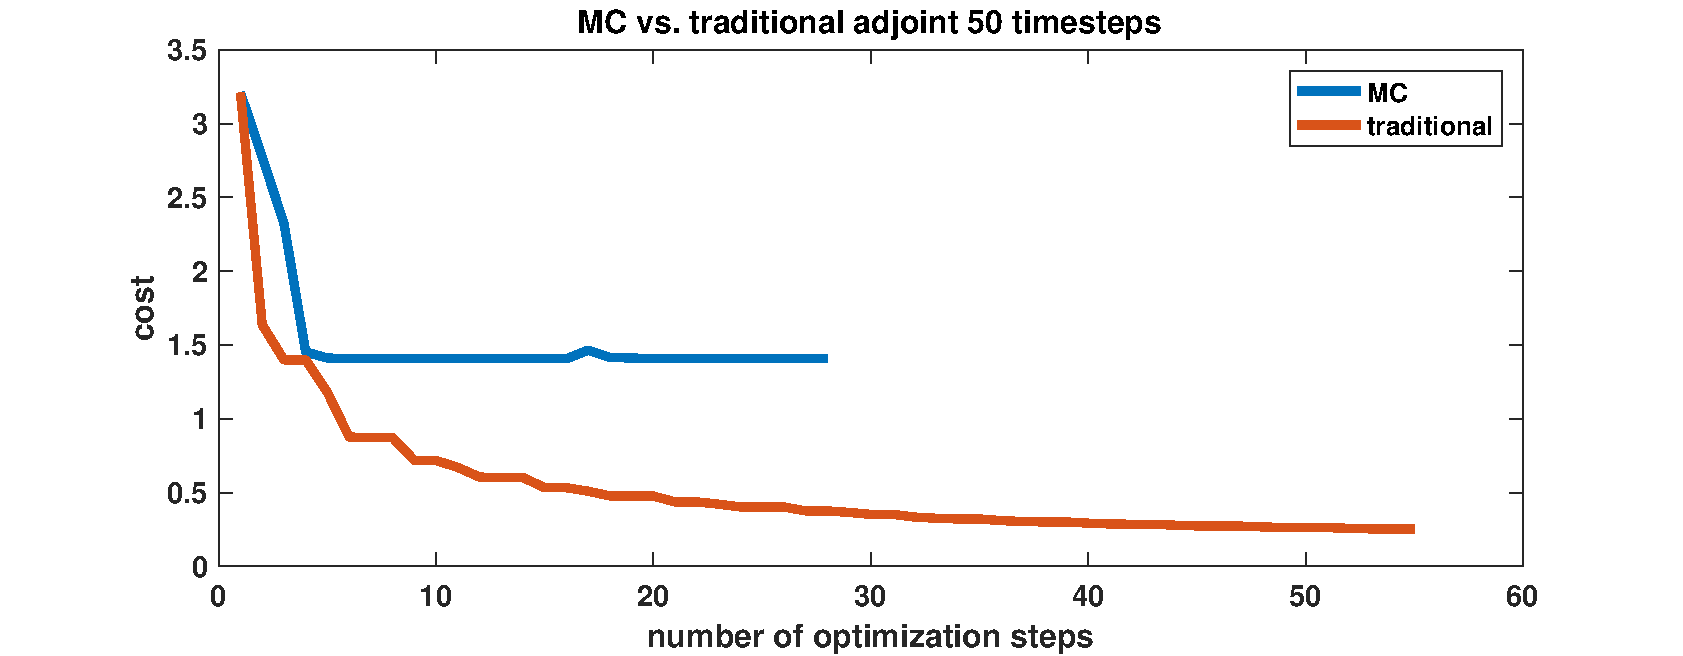
\includegraphics[width=\linewidth]{mctrad50}
	\caption{Sample run of the Monte-Carlo based optimizer, in orange (lower line) the optimization using the exact adjoint, in blue (upper line) the one approximating the gradient with Monte-Carlo.}
	\label{sampleRun}
\end{figure}
The Monte-Carlo based optimization stopped early because of a small gradient.
Another noteworthy characteristic is that the optimization problem seems to be hard:
The difference between Monte-Carlo and exact optimal costs is just one.
In conclusion, the preconditioner given by \eqref{preconditioner} is not satisfactory.

\section{Possible solutions}
\label{possibleSolutions}
A possible solution of the preconditioning dilemma could lie in using \emph{sequential Monte Carlo}
as described in \cite{sequential}, which relies on repeated application of the \emph{control variates} technique \cite{handbook} known for reducing the variance in Monte-Carlo simulations. This variant requires the eigenvalues of 
\begin{equation}
\lvert \mat{I} - \mat{PA} \rvert,
\end{equation}
to lie inside the unit circle where $\lvert \cdot \rvert$ denotes a componentwise magnitude.
This is fulfilled for our choice of preconditioner $\mat{P}$.
Moreover, sequential Monte-Carlo guarantees the variance of the random walks to be exponentially decreasing with the number of iterations, as long as the number of random walks per iteration is high enough.

A recent alternative seems to be \cite{multiway}, where the transition matrix of the random walks can vary over time. 
This approach requires the same prerequisites as sequential Monte-Carlo, but needs to have the full iteration matrix $\mat{I} - \mat{PA}$ to build the transition hypermatrix.
This is not feasible for the adjoint system of equations and would need a workaround.

\appendix

\subsection{Computing the derivatives for the Monte-Carlo adjoint solver}
\label{quantitiesNeeded}

The nonzero derivatives for the diagonal blocks are given by
\begin{align}
\pdiff{\Pi_K^{(i)}}{p_K^{(i)}} &= T_E^{(i-1)} + T_W^{(i-1)} + T_N^{(i-1)} + T_S^{(i-1)} \\
\pdiff{\Pi_K^{(i)}}{p_R^{(i)}} &= -T_E^{(i-1)} \\
\pdiff{\Pi_K^{(i)}}{p_L^{(i)}} &= -T_W^{(i-1)} \\
\pdiff{\Pi_K^{(i)}}{p_N^{(i)}} &= -T_U^{(i-1)} \\
\pdiff{\Pi_K^{(i)}}{p_S^{(i)}} &= -T_D^{(i-1)}
\end{align}
for cells which are not nearest to the well

and by
\begin{align}
\pdiff{\Sigma_K^{(i)}}{S_K^{(i)}} &= 1 \\
\pdiff{\Sigma_K^{(i)}}{{S_{\text{w}}}_K^{(i-1)}} &=  -1 + f^\prime({S_{\text{w}}}_K^{(i-1)}) \frac{\Delta t}{h}\cdot \biggr(\indicator(v_\text{tot, x}\lvert_E > 0) v_\text{tot, x}\lvert_E \\&- \indicator(v_\text{tot, x}\lvert_W < 0) v_\text{tot, x}\lvert_W + \indicator(v_\text{tot, y}\lvert_N > 0) v_\text{tot, y}\lvert_N  \nonumber\\&- \indicator(v_\text{tot, y}\lvert_S < 0) v_\text{tot, y}\lvert_S\biggr) \nonumber\\ &+\frac{\Delta t}{h}\cdot\biggr(-f({S_{\text{w}}}_K^{(i-1)})\lvert_E \pdiff{\hmean}{b}(\nonumber\\&\lambda_{\text{tot, }R}, \lambda_{\text{tot, }K}) \pdiff{\lambda}{S_\text{w}}\lvert_K \ddiff{p}{x}\lvert_E\pm \ldots\biggr) \nonumber\\
\pdiff{\Sigma_K^{(i)}}{{S_{\text{w}}}_R^{(i-1)}} &= f^\prime({S_{\text{w}}}_R^{(i-1)}) \frac{\Delta t}{h}\cdot \indicator(v_\text{tot, x}\lvert_E < 0) v_\text{tot, x}\lvert_E \nonumber\\&- \frac{\Delta t}{h} \pdiff{\hmean}{b}(\lambda_{\text{tot, }K}, \lambda_{\text{tot, }R}) \pdiff{\lambda}{S_\text{w}}\lvert_R \ddiff{p}{x}\lvert_E
\end{align}
%\pdiff{\Sigma_K^{(i)}}{{S_{\text{w}}}_L^{(i-1)}} &= -f^\prime({S_{\text{w}}}_L^{(i-1)}) \frac{\Delta t}{h}\cdot \indicator(v_\text{tot, x}\lvert_W > 0) v_\text{tot, x}\lvert_W \nonumber\\&+ \frac{\Delta t}{h} \pdiff{\hmean}{b}(\lambda_{\text{tot, }K}, \lambda_{\text{tot, }}) \pdiff{\lambda}{S_\text{w}}\lvert_R \ddiff{p}{x}\lvert_E
%\pdiff{\Sigma_K^{(i)}}{{S_{\text{w}}}_U^{(i-1)}} &= f^\prime({S_{\text{w}}}_U^{(i-1)}) \frac{\Delta t}{h}\cdot \indicator(v_\text{tot, y}\lvert_N < 0) v_\text{tot, y}\lvert_N \\
%\pdiff{\Sigma_K^{(i)}}{{S_{\text{w}}}_D^{(i-1)}} &= -f^\prime({S_{\text{w}}}_D^{(i-1)}) \frac{\Delta t}{h}\cdot \indicator(v_\text{tot, y}\lvert_S > 0) v_\text{tot, x}\lvert_S,
where
\begin{align}
f^\prime(S_\text{w}) &=  \frac{2\mu_\text{o}\mu_\text{w} (1 - S_\text{w})S_\text{w}}{\phi \cdot \left(\mu_\text{w}(1 - S_\text{w})^2 + \mu_\text{o}S_\text{w}^2\right)^2}\\
\indicator(b) &= \begin{cases} 1, &\text{if } b \text{ true} \\ 0, &\text{otherwise.}
\end{cases}
\end{align}

For the off diagonal blocks, we have
\begin{align}
\pdiff{\Sigma_K^{(i)}}{p_K^{(i)}} &= +\frac{\Delta t}{h^2} \biggr(T_E^{(i-1)} f(S_\text{w}^{(i-1)})\lvert_E \\&+ T_W^{(i-1)} f(S_\text{w}^{(i-1)})\lvert_W \nonumber\\&+ T_N^{(i-1)} f(S_\text{w}^{(i-1)})\lvert_N \nonumber\\&+T_S^{(i-1)}  f(S_\text{w}^{(i-1)})\lvert_S\biggr) \nonumber\\
\pdiff{\Sigma_K^{(i)}}{p_R^{(i)}} &= -\frac{\Delta t}{h^2}T_E^{(i-1)} f(S_\text{w}^{(i-1)})\lvert_E \\
\pdiff{\Sigma_K^{(i)}}{p_L^{(i)}} &= -\frac{\Delta t}{h^2}T_W^{(i-1)} f(S_\text{w}^{(i-1)})\lvert_W \\\\
\pdiff{\Sigma_K^{(i)}}{p_U^{(i)}} &= -\frac{\Delta t}{h^2}T_N^{(i-1)} f(S_\text{w}^{(i-1)})\lvert_N \\
\pdiff{\Sigma_K^{(i)}}{p_D^{(i)}} &= -\frac{\Delta t}{h^2}T_S^{(i-1)} f(S_\text{w}^{(i-1)})\lvert_S,
\end{align}
for cells not nearest to the well and
\begin{align}
\pdiff{\Pi_K^{(i)}}{{S_\text{w}}_K^{(i-1)}} &= 2 \pdiff{\lambda_\text{tot}^{(i-1)}}{S_\text{w}}\lvert_K\\&\sum_{n\in\{U, D, L, R\}} \frac{(p_K^{(i-1)} - p_n^{(i-1)}) \cdot (\lambda_{\text{tot, }n}^{(i-1)})^2}{(\lambda_{\text{tot, }K}^{(i-1)} + \lambda_{\text{tot, }n}^{(i-1)})^2} \nonumber\\
\pdiff{\Pi_K^{(i)}}{{S_\text{w}}_R^{(i-1)}} &= 2 \pdiff{\lambda_\text{tot}^{(i-1)}}{S_\text{w}}\lvert_R \cdot
\frac{(p_K^{(i-1)} - p_R^{(i-1)}) \cdot (\lambda_{\text{tot, }K}^{(i-1)})^2}{(\lambda_{\text{tot, }K}^{(i-1)} + \lambda_{\text{tot, }R}^{(i-1)})^2} \\
\pdiff{\Pi_K^{(i)}}{{S_\text{w}}_L^{(i-1)}} &= 2 \pdiff{\lambda_\text{tot}^{(i-1)}}{S_\text{w}}\lvert_L \cdot
\frac{(p_K^{(i-1)} - p_L^{(i-1)}) \cdot (\lambda_{\text{tot, }K}^{(i-1)})^2}{(\lambda_{\text{tot, }K}^{(i-1)} + \lambda_{\text{tot, }L}^{(i-1)})^2} \\
\pdiff{\Pi_K^{(i)}}{{S_\text{w}}_U^{(i-1)}} &= 2 \pdiff{\lambda_\text{tot}^{(i-1)}}{S_\text{w}}\lvert_U \cdot
\frac{(p_K^{(i-1)} - p_U^{(i-1)}) \cdot (\lambda_{\text{tot, }K}^{(i-1)})^2}{(\lambda_{\text{tot, }K}^{(i-1)} + \lambda_{\text{tot, }U}^{(i-1)})^2} \\
\pdiff{\Pi_K^{(i)}}{{S_\text{w}}_D^{(i-1)}} &= 2 \pdiff{\lambda_\text{tot}^{(i-1)}}{S_\text{w}}\lvert_D \cdot
\frac{(p_K^{(i-1)} - p_D^{(i-1)}) \cdot (\lambda_{\text{tot, }K}^{(i-1)})^2}{(\lambda_{\text{tot, }K}^{(i-1)} + \lambda_{\text{tot, }D}^{(i-1)})^2}
\end{align}
where
\begin{align}
\pdiff{\lambda_\text{tot}}{S_\text{w}} &= 2k\left(\frac{S_\text{w} - 1}{\mu_\text{o}} + \frac{S_\text{w}}{\mu_\text{w}}\right).
\end{align}

For solving the adjoint equations, we also need the derivatives of the residuals with respect to the parameters, in our case $\ln(k).$

For the pressure residuals and if $K$ is not the cell at the well, those read\\
\begin{align}
\pdiff{\Pi_K^{(i)}}{\ln(k)_K} &= \lambda^{(i-1)}\lvert_K\sum_{n\in\{L, R, U, D\}} (p_K^{(i)} - p_n^{(i)})\pdiff{\hmean}{b}(\lambda^{(i-1)}\lvert_n,\\& \lambda_\text{tot}^{(i-1)}\lvert_K)\nonumber\\
\pdiff{\Pi_K^{(i)}}{\ln(k)_L} &= (p_K^{(i)} - p_L^{(i)})\lambda_\text{tot}^{(i-1)}\lvert_L \pdiff{\hmean}{b}(\lambda_\text{tot}^{(i-1)}\lvert_K, \lambda_\text{tot}^{(i-1)}\lvert_L) \\
\pdiff{\Pi_K^{(i)}}{\ln(k)_R} &= (p_K^{(i)} - p_R^{(i)})\lambda_\text{tot}^{(i-1)}\lvert_R \pdiff{\hmean}{b}(\lambda_\text{tot}^{(i-1)}\lvert_K, \lambda_\text{tot}^{(i-1)}\lvert_R) \\
\pdiff{\Pi_K^{(i)}}{\ln(k)_U} &= (p_K^{(i)} - p_U^{(i)})\lambda_\text{tot}^{(i-1)}\lvert_U \pdiff{\hmean}{b}(\lambda_\text{tot}^{(i-1)}\lvert_K, \lambda_\text{tot}^{(i-1)}\lvert_U) \\
\pdiff{\Pi_K^{(i)}}{\ln(k)_D} &= (p_K^{(i)} - p_D^{(i)})\lambda_\text{tot}^{(i-1)}\lvert_D \pdiff{\hmean}{b}(\lambda_\text{tot}^{(i-1)}\lvert_K, \lambda_\text{tot}^{(i-1)}\lvert_D)
\end{align}

where 
\begin{equation}
\pdiff{\hmean}{b}(a, b) := \frac{2a^2}{(a+b)^2}.
\end{equation}

On the other hand, the saturation residuals $\Sigma_K$ lead to the following derivatives

\begin{align}
\pdiff{\Sigma_K}{\ln(k)_K} &= \lambda_{\text{tot}}^{(i-1)}\lvert_K \frac{\Delta t}{h} \biggr(\\&(f(S_\text{w}^{(i-1)})v_{\text{tot }, x}^{(i-1)})\lvert_E\pdiff{\hmean}{b}(\lambda_\text{tot}^{(i-1)}\lvert_E, \lambda_\text{tot}^{(i-1)}\lvert_K) \nonumber\\&\cdot(-\ddiff{p}{x}\rvert_E)  \nonumber\\&- (f(S_\text{w}^{(i-1)})v_{\text{tot }, x}^{(i-1)})\lvert_W\pdiff{\hmean}{b}(\lambda_\text{tot}^{(i-1)}\lvert_W, \lambda_\text{tot}^{(i-1)}\lvert_K)\nonumber\\&\cdot(-\ddiff{p}{x}\rvert_W) \nonumber\\&+ (f(S_\text{w}^{(i-1)})v_{\text{tot }, y}^{(i-1)})\lvert_N\pdiff{\hmean}{b}(\lambda_\text{tot}^{(i-1)}\lvert_N, \lambda_\text{tot}^{(i-1)}\lvert_K)\nonumber\\&\cdot(-\ddiff{p}{y}\rvert_N)\nonumber\\&- (f(S_\text{w}^{(i-1)})v_{\text{tot }, y}^{(i-1)})\lvert_S\pdiff{\hmean}{b}(\lambda_\text{tot}^{(i-1)}\lvert_E, \lambda_\text{tot}^{(i-1)}\lvert_S)\nonumber\\&\cdot(-\ddiff{p}{y}\rvert_S)\nonumber\\&\biggr) \nonumber \\
\pdiff{\Sigma_K}{\ln(K)_R} &= \lambda_{\text{tot}}^{(i-1)}\lvert_R \frac{\Delta t}{h} f(S_\text{w}^{(i-1)})v_{\text{tot }, x}^{(i-1)})\lvert_E\nonumber\\&\cdot\pdiff{\hmean}{b}(\lambda_\text{tot}^{(i-1)}\lvert_K, \lambda_\text{tot}^{(i-1)}\lvert_E)(-\ddiff{p}{x}\rvert_E)\\
\pdiff{\Sigma_K}{\ln(K)_L} &= -\lambda_{\text{tot}}^{(i-1)}\lvert_L\frac{\Delta t}{h} f(S_\text{w}^{(i-1)})v_{\text{tot }, x}^{(i-1)})\lvert_W\nonumber\\&\cdot\pdiff{\hmean}{b}(\lambda_\text{tot}^{(i-1)}\lvert_K, \lambda_\text{tot}^{(i-1)}\lvert_L)\cdot(-\ddiff{p}{x}\rvert_W)\\
\pdiff{\Sigma_K}{\ln(K)_U} &= \lambda_{\text{tot}}^{(i-1)}\lvert_U \frac{\Delta t}{h} f(S_\text{w}^{(i-1)})v_{\text{tot }, x}^{(i-1)})\lvert_N\nonumber\\&\cdot\pdiff{\hmean}{b}(\lambda_\text{tot}^{(i-1)}\lvert_K, \lambda_\text{tot}^{(i-1)}\lvert_U)\cdot(-\ddiff{p}{y}\rvert_N)\\
\pdiff{\Sigma_K}{\ln(K)_D} &= -\lambda_{\text{tot}}^{(i-1)}\lvert_D\frac{\Delta t}{h} f(S_\text{w}^{(i-1)})v_{\text{tot }, x}^{(i-1)})\lvert_S\nonumber\\&\cdot\pdiff{\hmean}{b}(\lambda_\text{tot}^{(i-1)}\lvert_K, \lambda_\text{tot}^{(i-1)}\lvert_D)(-\ddiff{p}{y}\rvert_S)
\end{align}



\bibliographystyle{IEEEtran}
\bibliography{references}


\end{document}
